\documentclass[tikz,border=2pt]{standalone}
\usepackage{amsmath,amssymb}
\usepackage{tikz}
\usetikzlibrary{arrows.meta}

\begin{document}
% Near x0 a differentiable map f is approximated by the linear map with matrix Jf(x0): a tiny
% square at x0 is sent to a tiny parallelogram at f(x0), spanned by the columns of Jf(x0).
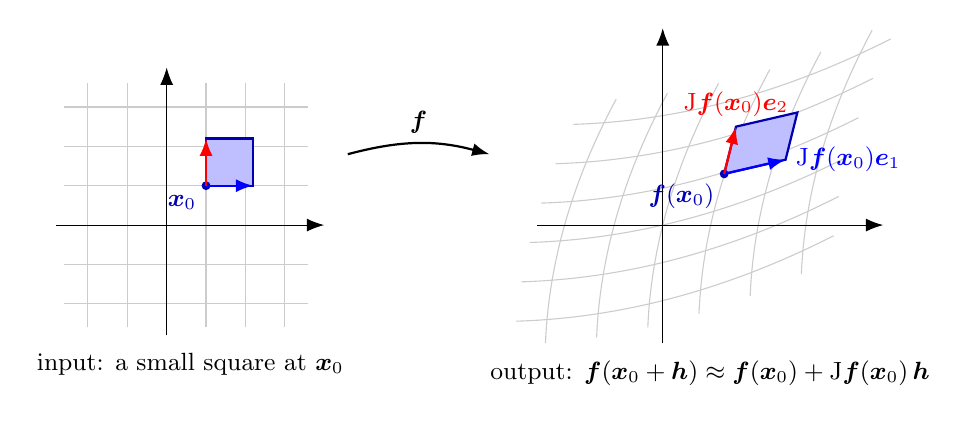
\begin{tikzpicture}[every node/.style={font=\small}, >={Latex[length=2.2mm]}]
	\begin{scope}
		\draw[gray!40, step=0.5] (-1.3,-1.3) grid (1.8,1.8);
		\draw[->] (-1.4,0) -- (2.0,0); \draw[->] (0,-1.4) -- (0,2.0);
		\fill[blue!25, draw=blue!70!black, thick] (0.5,0.5) rectangle (1.1,1.1);
		\fill[blue!70!black] (0.5,0.5) circle (1.6pt) node[below left] {$\boldsymbol{x}_0$};
		\draw[->, blue, thick] (0.5,0.5) -- (1.1,0.5); \draw[->, red, thick] (0.5,0.5) -- (0.5,1.1);
		\node[anchor=north] at (0.3,-1.5) {input: a small square at $\boldsymbol{x}_0$};
	\end{scope}
	\draw[->, thick] (2.3,0.9) to[bend left=15] node[above] {$\boldsymbol{f}$} (4.1,0.9);
	\begin{scope}[xshift=6.3cm]
		% curved image grid
		\foreach \u in {-1.0,-0.5,...,1.5} {\draw[gray!40] plot[domain=-1.3:1.8, samples=30] ({\u*1.3+0.25*\x+0.08*\x*\x},{\x*1.0+0.3*\u+0.1*\u*\u});}
		\foreach \v in {-1.0,-0.5,...,1.5} {\draw[gray!40] plot[domain=-1.3:1.8, samples=30] ({\x*1.3+0.25*\v+0.08*\v*\v},{\v*1.0+0.3*\x+0.1*\x*\x});}
		\draw[->] (-1.6,0) -- (2.8,0); \draw[->] (0,-1.5) -- (0,2.5);
		% image of the square: parallelogram spanned by columns (1.3,0.3) and (0.25,1.0) scaled by 0.6, at f(x0)
		\fill[blue!25, draw=blue!70!black, thick] (0.78,0.65) -- (1.56,0.83) -- (1.71,1.43) -- (0.93,1.25) -- cycle;
		\fill[blue!70!black] (0.78,0.65) circle (1.6pt) node[below left] {$\boldsymbol{f}(\boldsymbol{x}_0)$};
		\draw[->, blue, thick] (0.78,0.65) -- (1.56,0.83) node[right] {$\mathrm{J}\boldsymbol{f}(\boldsymbol{x}_0)\boldsymbol{e}_1$};
		\draw[->, red, thick] (0.78,0.65) -- (0.93,1.25) node[above] {$\mathrm{J}\boldsymbol{f}(\boldsymbol{x}_0)\boldsymbol{e}_2$};
		\node[anchor=north] at (0.6,-1.6) {output: $\boldsymbol{f}(\boldsymbol{x}_0+\boldsymbol{h})\approx\boldsymbol{f}(\boldsymbol{x}_0)+\mathrm{J}\boldsymbol{f}(\boldsymbol{x}_0)\,\boldsymbol{h}$};
	\end{scope}
\end{tikzpicture}
\end{document}
